\begin{frame}
	\centering \LARGE \color{naranjaUCA} Modelo de cola M/M/1/c
			\begin{center}
				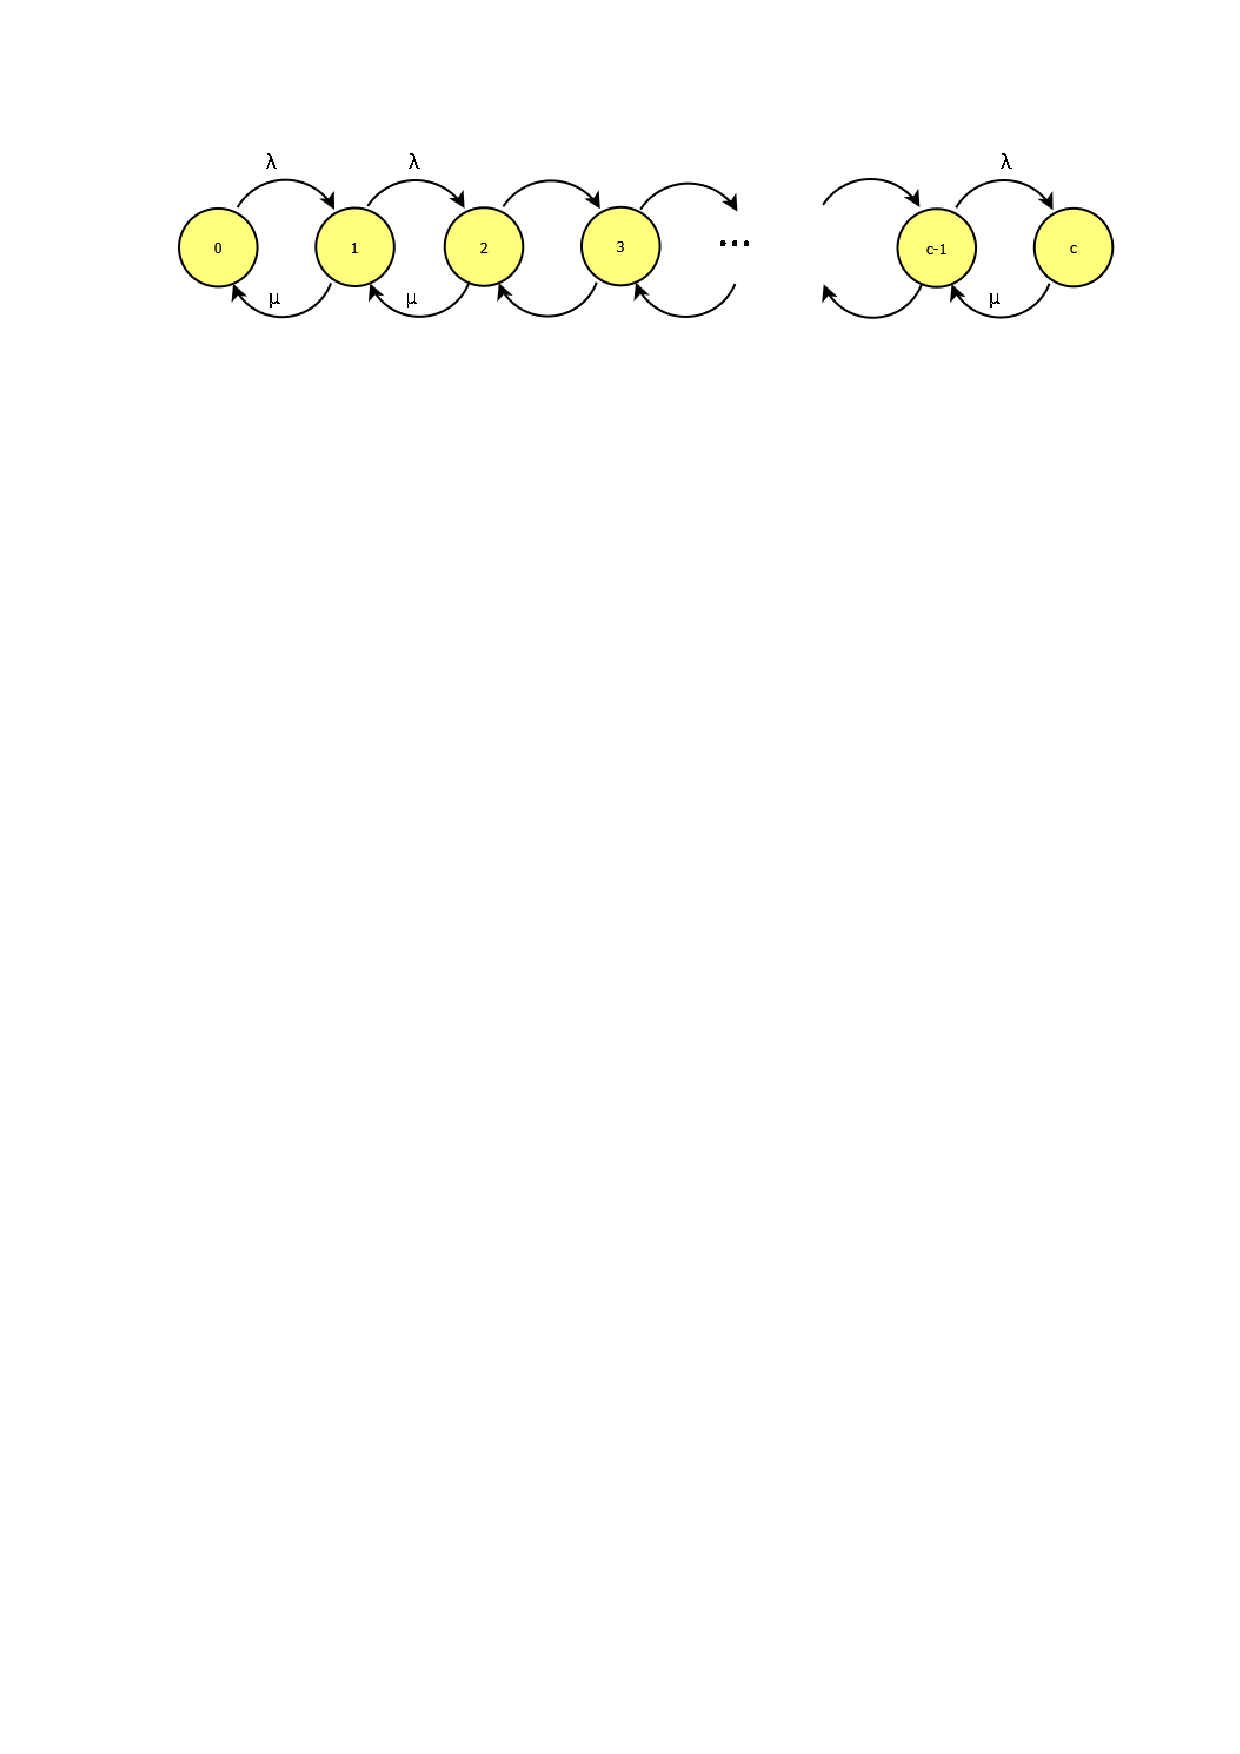
\includegraphics[trim = 10mm 220mm 10mm 25mm, clip,width=0.9\linewidth]{MMc}
			\end{center}
\end{frame}
\begin{frame}{M/M/1/c}

	Podemos modelar esta cola como un proceso de nacimiento-muerte con los siguientes parámetros: \pause
		$$\begin{array}{cc}
		\lambda_j=\lambda & (j=0,1,...,c-1)\\ \pause
		\lambda_c=0 & \\ \pause
		\mu_0=0 &  \\ \pause
		\mu_j=\mu &  (j=1,2,...,c)\\
		\end{array}$$
\end{frame}
\begin{frame}{M/M/1/c}
	Cuyas ecuaciones de balance serán: \pause
		$$\begin{array}{cc}
		\pi_0=\frac{1-\rho}{1-\rho^{c+1}} & \\ \pause
		\pi_j=\rho^j\pi_0 & (j=1,2,...,c)\\ \pause
		\pi_j=0 & (j=c+1,c+2,...)\\ \pause
		\end{array}$$
\end{frame}
\begin{frame}{M/M/1/c}
		\begin{block}{Cálculo de L}
	\begin{itemize}
		\item  Si $\rho=1$ tenemos que  \pause
		$$\begin{array}{cc}
		\pi_j=\frac{1}{c+1} & (j=0,1,...,c)\\ 
		
		L=\sum_{k=0}^{k=c}k\pi_k=\frac{c}{2}& \\
		\end{array}$$ \pause
		
		\item Si $\rho\neq1$ \pause
		\begin{center}
			$L=\sum_{k=0}^{c}k\frac{\rho^k (1-\rho)}{1-\rho^{c+1}}=...=\frac{\rho}{1-\rho}-\frac{(c+1)\rho^{c+1}}{1-\rho^{c+1}}$
		\end{center}
	
		\end{itemize}
	\end{block}
\end{frame}
\begin{frame}{M/M/1/c}
	
	\begin{itemize}
	\item 	$$L_s=1-\pi_=0$$  \pause
	\item  $$L_q=L-L_s=L-1+\pi_=0$$
	\end{itemize}
\end{frame}
\begin{frame}{M/M/1/c}
		\begin{block}{Cálculo de W}
	Como tiene capacidad finita no todas las personas podrán entrar en el sistema. El ratio de clientes que verdaderamente entrarán será:
	\pause
	\\
	 $\lambda-\lambda\pi_c=\lambda(1-\pi_c)$ \pause
	 \\
	 Usando las fórmulas de Little:
	\begin{itemize}
		\item $W=\frac{L}{\lambda(1-\pi_0}$ \pause
		\item $W_q=\frac{L_q}{\lambda(1-\pi_c)}$ \pause
		\item $W_s=\frac{1}{\mu}$ \pause
	\end{itemize}
\end{block}
\end{frame}